\pagenumbering{arabic}
\section{项目描述}
据统计,世界上总共有超过10,000种鸟类.从人迹罕至的雨林到郊区甚至是城市,几乎一切环境当中都可以找到它们.鸟类在自然界中起着至关重要的作用.它们在食物链中处于较高的位置,并且整合了较低级别发生的变化.故而,鸟类是环境质量以及生态多样性的重要指标.

通过鸟类的鸣叫来观察鸟类比直接观察鸟类更为容易.通过对鸟类的声音进行检测,可以让我们直接获取鸟类种类,数量等重要信息.

在实际对鸟类鸣叫数据的处理中,传统上需要通过领域专家进行手动处理.但是这样的分析往往是十分缓慢的,并且结果也并不十分可靠.

机器学习为鸟类鸣叫数据处理提供了新的思路.通过对现成的鸟鸣数据集(标签完备的)的学习,我们能够达到\textbf{检测连续录音中鸟鸣,以及分辨鸟鸣对应鸟类名称的目的}.


\subsection{原始数据源}
\begin{itemize}
	\item 鸟鸣训练集: 来自\href{https://www.xeno-canto.org/}{xeno-canto}.
	\begin{figure}[thbp!]
		\centering
		
\includegraphics[scale=0.6]{figure/xc}
	\end{figure}
	可以通过Kaggle获取.数据集大致情况可视化如下所示:
	\begin{figure}[thbp!]
		\centering
		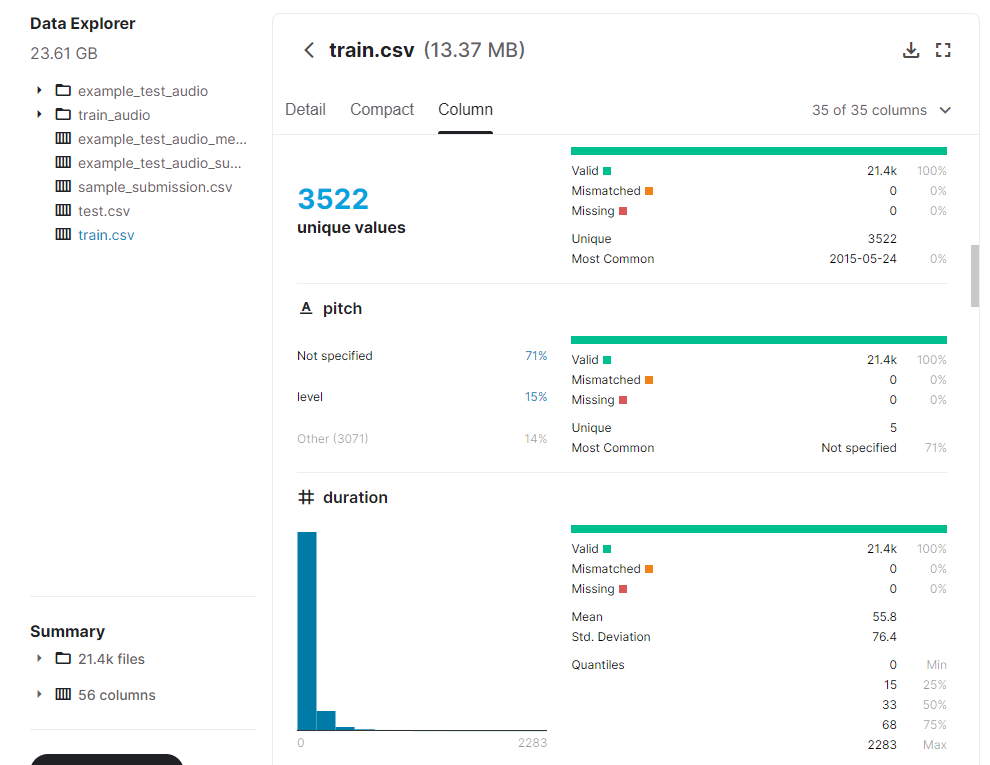
\includegraphics[scale=0.3]{figure/data}
		\caption{Kaggle: Cornell Birdcall Identification的数据集}
	\end{figure}
	\item 鸟类图像网站: 来自\href{https://ebird.org/home}{ebird.org}.由于网站未提供可下载的汇总文件,所以自行编写Python爬虫小程序以爬取:
	\begin{figure}[thbp!]
	\centering
	
\includegraphics[scale=0.4]{figure/ebird}
	\end{figure}
	\begin{lstlisting}[language=python,breaklines=true]
import urllib
import requests
import pandas as pd
from lxml import etree
from pathlib import Path

# 准备路径
ROOT = Path("C:/Users/TsuiPo/Downloads/Compressed")
PICPATH = ROOT / "bird_pic"
TRAIN = ROOT / "train.csv"
# 读取列表
train = pd.read_csv(str(TRAIN))
birds = train["ebird_code"].unique()
# 构造url
urls = ["https://ebird.org/species/{}/".format(bird) for bird in birds]


headers = {"User-Agent": "Mozilla/5.0 (Windows NT 10.0; Win64; x64) AppleWebKit/537.36 (KHTML, like Gecko) Chrome/90.0.4430.93 Safari/537.36",}
for i in range(len(urls)):
print("---Crawling bird: " + birds[i] + "---")
r = requests.get(urls[i], headers=headers)
page = etree.HTML(r.content)
image_url = page.xpath(r'//*[@id="MediaFeed-showcase"]/figure[1]/a/div/img/@src')[0]
SAVE_PATH = PICPATH / Path(birds[i] + '.jpg')

# b_image = requests.get(image_url, headers=headers)
request = urllib.request.Request(image_url, headers=headers)
response = urllib.request.urlopen(request)
img = response.read() # 存放二进制图片
print(">正在下载:" + birds[i])
try:
with open(str(SAVE_PATH), 'wb') as f:
f.write(img)
print(">抓取成功!")
except:
print(">下载错误...")
	\end{lstlisting}
	图片下载到本地,如下所示:
	\begin{figure}[thbp!]
		\centering
		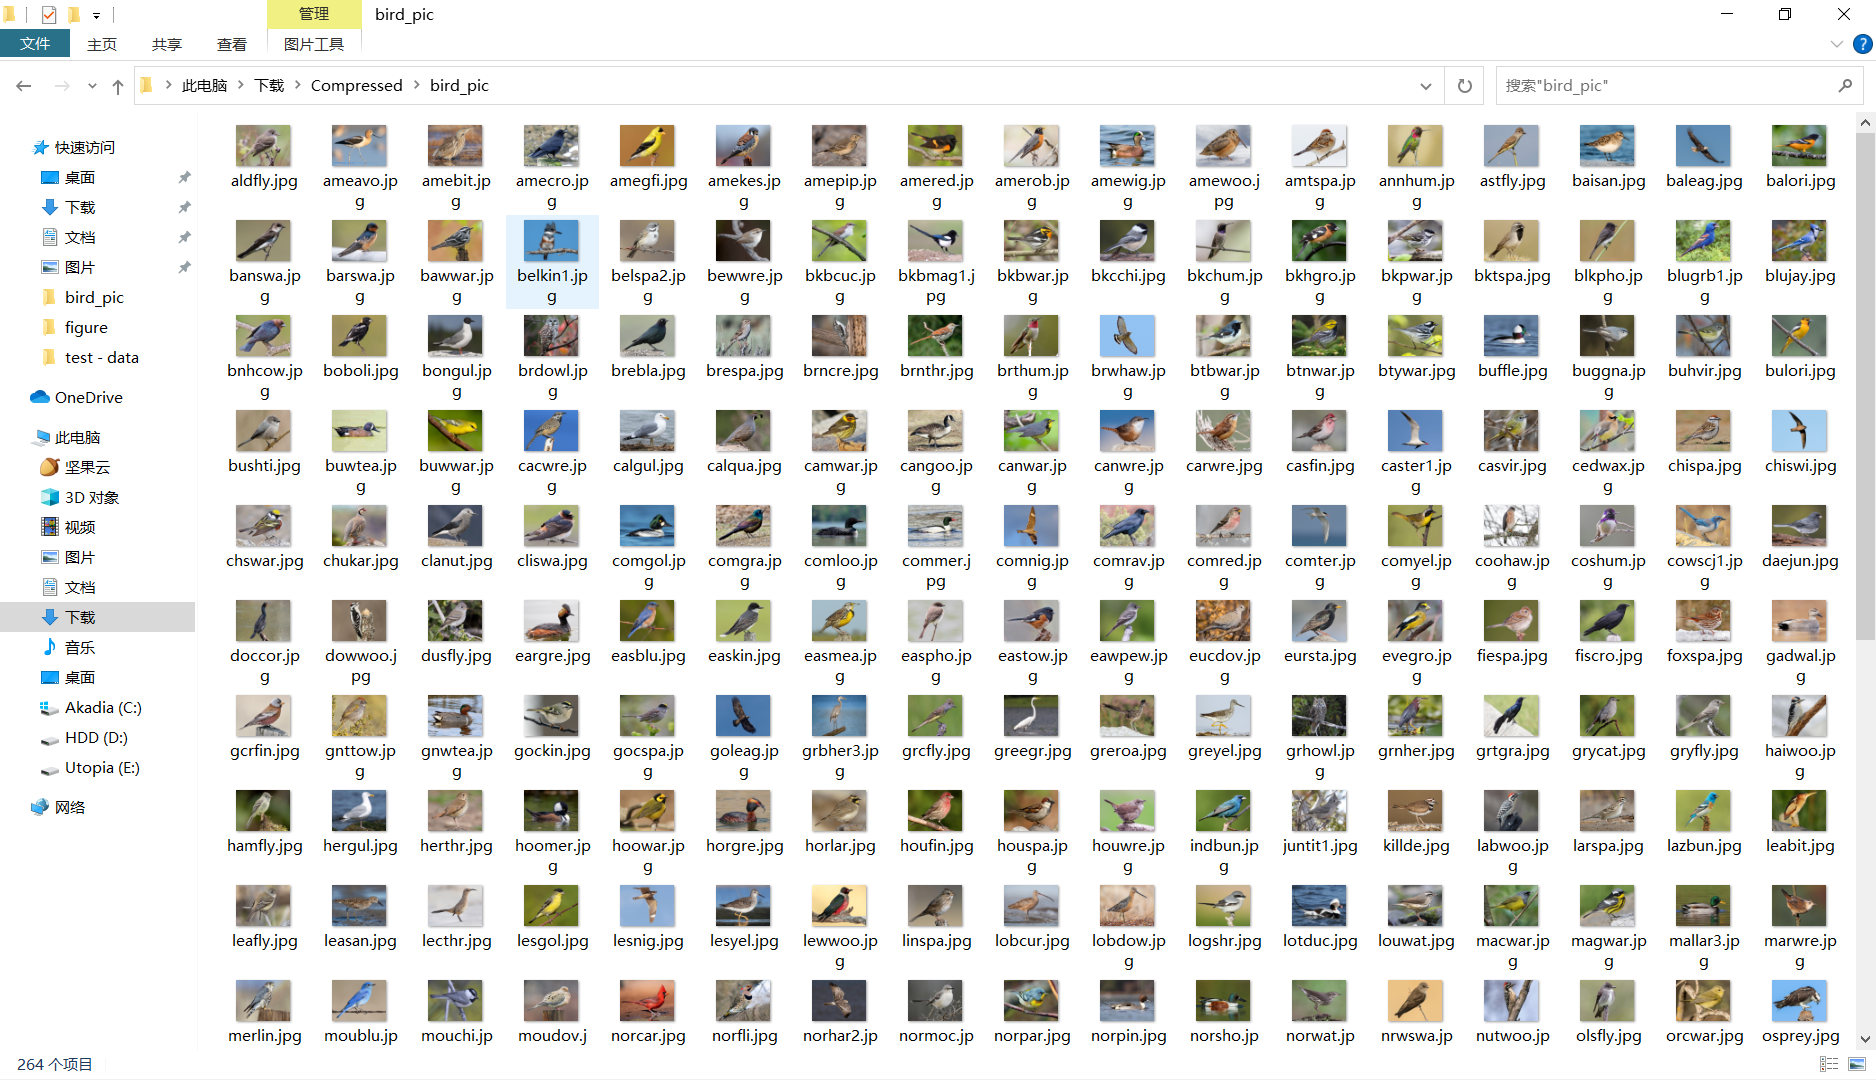
\includegraphics[scale=0.2]{figure/birds}
		\caption{图片爬取后暂时存放本地}
	\end{figure}
\end{itemize}


